% scheme representing the bounds
% expresed in paper Renner+Wolf 2003
% on the quantities intrinsic information,
% secret key rate and information of formaion
\usetikzlibrary{calc}
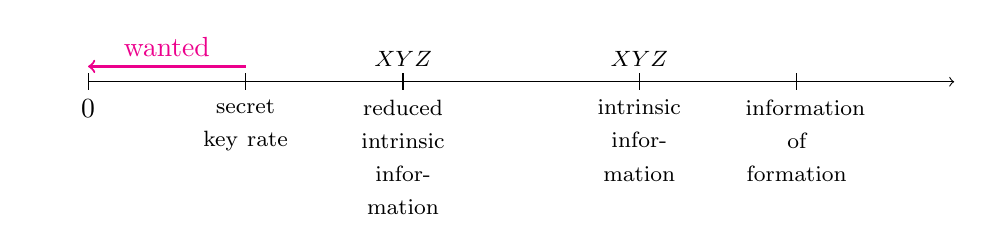
\begin{tikzpicture}

\tikzset{
    position label/.style={
       below = 3pt,
       align=center,
%       text height = 1.5ex,
%       text depth = 1ex,
       text width=13mm
    },
   brace/.style={
     decoration={brace},
     decoration={raise=3ex},
     decorate
   },
   blabel/.style={
		above = 13pt,
		align=center,
		pos=0.5   
   }
}

% draw horizontal line
\draw[->] (0,0) -- (11,0);

%draw vertical lines
\foreach \x in {0,2,4,7,9}
   \draw (\x cm,3pt) -- (\x cm,-3pt);

%labels
\node [position label] (Start) at (0,0) {$0$};
\node [position label] (skr) at (2,0) {\footnotesize secret key rate};
\node [position label] (rinf) at (4,0) {\footnotesize reduced intrinsic information};
\node [position label] (inf) at (7,0) {\footnotesize intrinsic information};
\node [position label] (iof) at (9,0) {\footnotesize information of formation};

\node (eqrinf) at ($(rinf.north) + (0,0.4)$) {\footnotesize $\redintrinfo{X}{Y}{Z}$};
\node (eqinf) at ($(inf.north) + (0,0.4)$) {\footnotesize $\intrinfo{X}{Y}{Z}$};

%\draw [brace] (skr.north) -- node [blabel] {\footnotesize arbitrarily large} (inf.north);
\draw [->, thick, magenta] ($(skr.north)+(0,0.3)$) -- node [above] {wanted} ($(Start.north)+(0,0.3)$);
%\draw [->, thick, magenta, dashed] ($(rinf.north)+(0,0.3)$) to [out=10,in=90] ($(Start.north)+(0,0.3)$);
\end{tikzpicture}